\chapter{Vorgehensweise}
\reiter
Es war ursprünglich geplant RUP\footcite{Lehrunterlagen-RUP} als Vorgehensmethode zu verwenden. 
\section{RUP}
RUP steht für Rational Unified Process und ist ein Prozessmodell, dass für die Software-Entwicklung konzipiert wurde und einen besonderen Schwerpunkt auf objektorientierte Entwicklung legt. Das Prozessmodell wurde von der Firma Rational entwickelt und besteht seit 1998 als RUP. Vorgängermodelle gibt es seit 1995. 
RUP berücksichtigt Best-Practices der Softwareentwicklung, also, Richtlinien, die aus Jahrelanger Erfahrung in der Industrie abgeleitet werden konnten. Pest-Practices müssen nicht zwingend befolgt werden, stellen aber für Entwickler einen guten Ansatz, der durch Erfahrene Herausgeber definiert worden ist, dar. 
RUP orientiert sich an Anwendungsfällen, die Anforderungen an das Gesamtsystem beschreiben. Anforderungen können als größere und ausführlicher definierte User-Stories gesehen werden.  
Der Projektablauf ist in vier Phasen aufgeteilt. Nach jeder Phase wird ein Meilenstein definiert, der inhaltlich klar beschrieben wurde.
Um die Projektziele erreichen zu können werden verschiedene Prozesse, einen Workflow, die, während jeder Phase als Querschnittsaufgabe, durchgeführt werden müssen, benötigt. Ein Workflow beschreibt welches Teammitglied welche Aufgabe zu welcher Zeit mit einem bestimmten Ergebnis durchzuführen hat.
In jeder Phase erfolgt die Entwicklung in kurzen Zyklen, die Iterationen genannt werden. Die Arbeit in einer Iteration ist auf die Erfüllung von Meilensteinen fokussiert. Am Ende einer Iteration sollte immer eine funktionsfähige Version des zu entwickelten Systems stehen.
\newpage
\subsection{Phasen}
\begin{itemize}
	\item \textbf{Inception-Phase:} Abgrenzung des Projektumfangs und genaue Beschreibung der wesentlichen Ziele. Es wird die Machbarkeit analysiert und der Aufwand festgestellt.
	\item \textbf{Elaboration:} Wichtigste Phase im Projekt. Hier sollte eine vollständige Analyse des Systems vorliegen. Es soll am Ende dieser Phase ein Prototyp vorliegen, der die wichtigsten Anforderungen beinhaltet.
	\item \textbf{Construction:} Hier finden die Entwicklung und das Testen der Applikation/Features statt.
	\item \textbf{Transition:} In dieser Phase soll ein Prototyp vorhanden sein der dem Auftraggeber übergeben werden kann. 
\end{itemize}
\begin{center}
\begin{figure}[H]
	\centering
	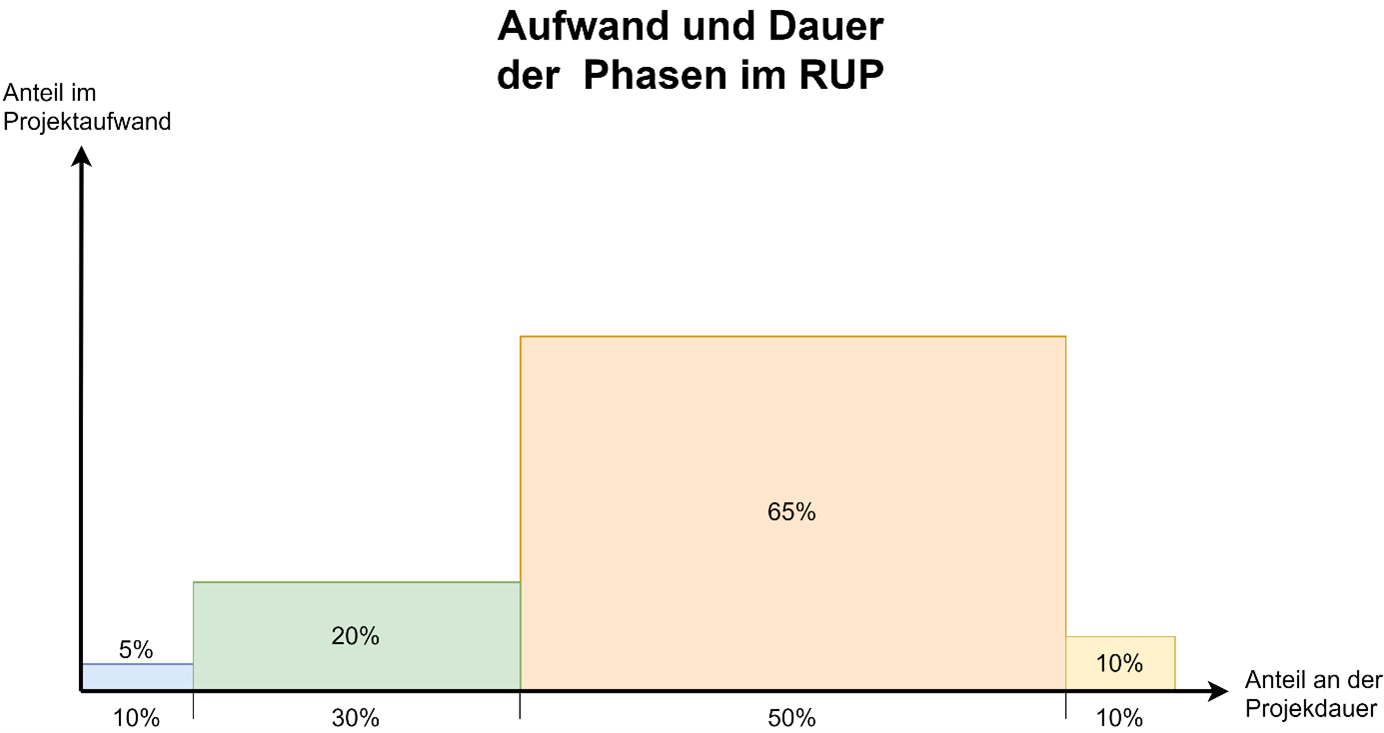
\includegraphics[width=\textwidth]{RUP-Arbeitsdauer.png}
	\caption{Verteilung des Arbeitsaufwandes bei RUP in Bezug auf die Phasen}
\end{figure}
\end{center}
Diese Phasen werden genauer durch Phasenergebnisse sowie Meilenstein-Kriterien, die bei dem Übergang in die nächste Phase erfüllt werden müssen, beschrieben.
Die Anzahl der Iterationen in einer Phase wird durch den Schwierigkeitsgrad des Projekts bestimmt. 
\subsection{Iterationen}
Die kurzen Entwicklungszyklen\footcite{rup-workflows} der Iterationen in RUP ermöglichen ein frühzeitiges Feedback des Kunden, was hilft, dass späte Änderungen durch den Kunden vermieden werden können. 
\begin{center}
\begin{figure}[H]
	\centering
	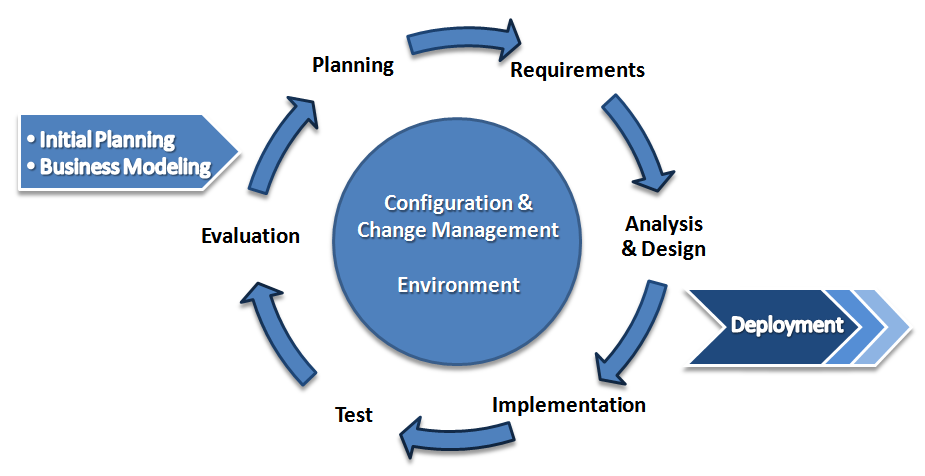
\includegraphics[width=\textwidth]{rup_iterationen.png}
	\caption{Iterationen in RUP}
\end{figure}
\end{center}
Die obenstehende Grafik zeigt alle Workflows einer Iteration. Die verschiedenen Workflows werden abhängig von der Phase der Iteration mit verschiedenen Intensitäten abgearbeitet. 
Es können mehrere Zyklen pro Iteration ablaufen.
Am Anfang jeder Iteration wird ein Iterationsplan erstellt, der die Aufgaben und Ziele einer jeden Iteration definiert. 
RUP trägt durch seine iterative Natur zur Vermeidung eines Late Design Breakages bei. Nicht iterative Modelle ermöglichen in einem frühen Stadium der Entwicklung keine Gesamtsicht auf das System. Mängel im System können erst spät erkannt werden. Somit müssen in vielen Komponenten der Software Änderungen vorgenommen werden, was einen hohen Aufwand darstellt und Verzögerungen im Deployment mit sich ziehen kann. 
Ein iterativer Entwicklungsansatz kann zwar nach jeder abgeschlossenen Phase auch Probleme offenlegen, diese sind aber auf Komponenten, die seit der zuletzt abgeschlossenen Phase erstellt wurden, begrenzt.
\subsection{Workflows}
\begin{itemize}
\item \textbf{Business Modelling:} Ein Business Model stellt die Geschäftsprozesse dar, für die Softwareentwickelt wird die diese umsetzt. Die Erstellung eines Business Models ist nicht zwingend notwendig.
\item \textbf{Requirements:} Es werden Anforderungen erstellt, die eine bessere Ansicht der zu entwickelnden Software ermöglichen soll. Diese Ansicht auf die Anforderungen des Projekts soll helfen, die Kommunikation zwischen Entwicklern und Stakeholdern, also Personen, die nicht im Entwicklerteam sind, wie zum Beispiel Kunden, zu vereinfachen.
\item \textbf{Analysis and Design:} Es wird der Systementwurf erstellt. Der Systementwurf ist ein Bauplan des Gesamtsystems, der die Entwicklung vereinfachen soll und allen Anforderungen der Funktionalität, Performance und Robustheit entspricht
\item \textbf{Implementation:} Es werden die Komponenten die im zuvor erarbeiteten Systemplan definiert wurden implementiert.
\item \textbf{Testing:} Die neu implementierten Komponenten werden getestet. Dieser Workflow findet im gesamten Projektverlauf statt.
\item \textbf{Deployment:} Stellt die Auslieferung an den Kunden dar. Es wird ein Release erstellt, gegebenenfalls beim Kunde installiert oder beim Umstieg des Kunden auf das neue vom alten System geholfen.
\end{itemize}
\subsection{Supporting Workflows}
\begin{itemize} 
	\item \textbf{Configuration and Change Management:} Kümmert sich um die Querschnittsaufgaben des Konfigurations- und Änderungsmanagements.
	\item \textbf{Project Management} 
	\item \textbf{Environment:} Anpassung des RUP an die sich ändernden Anforderungen im Projekt. Im Environment-Workflow werden auch alle Ressourcen, die zur Durchführung des Projekts benötigt werden zur Verfügung gestellt.
\end{itemize}
\section{SCRUM}
Im Rahmen der Anfangsarbeiten der Diplomarbeit wurde abteilungsintern die Verwendung der Projektmanagementsoftware Vivifyscrum vorgeschrieben. Durch diese Vorschrift konnte das Projekt nicht mit dem RUP-Prozessmodell entwickelt werden. 
Als Reaktion darauf wurde entschieden, dass SCRUM\footcite{Lehrunterlagen-SCRUM} als Prozessmodell verwendet werden soll.
\subsection{Rollen in Scrum}
Scrum hat grundsätzlich drei Rollen:
\begin{itemize} 
	\item \textbf{Product Owner:} dieser leitet das Projekt. Er vertritt das Team vor dem Auftraggeber, seine Aufgabe ist es die Erhebung, die Beschreibung und die Priorisierung der Anforderungen durchzuführen.
	\item \textbf{Scrum Master:} diese Person moderiert den Prozessablauf und versucht ihn voranzubringen. Er ist kein Mitglied des Entwicklungsteams.
	\item \textbf{Team} ist eine Gruppe von Entwicklern, die an dem Projekt arbeiten und für die Umsetzung der Arbeiten verantwortlich ist.
\end{itemize}
\begin{center}
\begin{figure}[H]
	\centering
	\includegraphics[width=\textwidth]{SCRUM-Verhältnisse.png}
	\caption{Visualisierung der Rollen in SCRUM}
\end{figure}
\end{center}
\subsection{Product Backlog}
Bei Scrum gibt es den sogenannten Product Backlog, er beinhaltet alle Anforderungen, diese werden nach und nach in Sprints abgearbeitet.
\subsection{Sprint Planning Meeting}
Im Sprint Planning Meeting wird besprochen was im nächsten Sprint das voraussichtliche Ziel ist. Der Product Owner wählt die Arbeitspakete aus, die am höchsten priorisiert sind und in dem Sprint abzuarbeiten sind. Hier nehmen Product Owner, Scrum Master und das Team teil. 
\subsection{Sprint}
Ein Sprint ist die Phase, in der die Softwareentwicklung abgewickelt wird. Dieser dauert meist ein bis vier Wochen. 
\subsection{Daily Scrum}
Das Daily Scrum ist ein täglich in der Früh stattfindendes Meeting. Es werden Aufgaben vom Product Owner an das Team vergeben. Die Dauer eines solchen Meeting soll ungefähr 15 Minuten dauern.
\subsection{Sprint Review}
Das Sprint Review Meeting wird am Ende jedes Sprints abgehalten. Es wird ein lauffähiger Prototyp vorgestellt und es wird besprochen, wie der Sprint hinsichtlich abgearbeiteter Arbeitspakete verlaufen ist. Das Endergebnis soll zeigen ob alle Erwartungen des Kunden erfüllt wurden.
\subsection{Sprint Retrospektive}
Hier wird mit dem Scrum Master besprochen, wie der Arbeitsprozess bis zu diesem Zeitpunkt verlaufen ist. Das Ergebnis einer Sprint Retrospektive sind Maßnahmen, die den Entwicklern helfen sollen, zukünftige Sprints besser abschließen zu können.
\subsection{Fortschrittskontrolle}
Die nachfolgenden Methoden unterstützen die Planung, Durchführung und die Kontrolle des Arbeitsfortschrittes.
\begin{itemize}
	\item	User Stories
	\item	Sprint Backlog
	\item	Burndown Chart
	\item	Timeboxing
	\item	Definition of Done
\end{itemize}
\subsection{User Stories}
Eine User Story gibt eine Anforderung vor. Der Kunde gibt unter Absprache mit dem Product Owner und dem Team alle User Stories am Anfang des Projekts an.
Anhand der User Stories kann der Fortschritt des Projekts gemessen werden.
Eine User Story ist eine zusammenfassende Einheit von ein oder mehreren Arbeitspaketen.
\subsection{Sprint Backlog}
Das Sprint Backlog stellt eine visuelle Darstellung dar, mit der der Fortschritt der Abarbeitung des Projekts dargestellt werden kann. Es werden auf einer Art Pinwand die User Stories, die im Sprint sind aufgelistet. Diese User Stories werden dann weiter in ihre Arbeitspakete aufgeteilt und können einen von drei Status, „offen“, „in Arbeit“ und „fertig“ haben.
\subsection{Burndown Chart}
Beim Burndown Chart wird der Verlauf des Projekts an den abgearbeiteten Tasks gemessen und bildlich dargestellt. In dem Diagramm beschreibt die x-Achse den Aufwand (in Personenstunden) bzw. die Anzahl von Tasks und die y-Achse die Arbeitstage des Sprints. 
Hierbei gibt es mehrere Linien, an denen der Fortschritt gemessen wird. Eine gibt die ideale Abarbeitung der Tasks an, eine den aktuellen Fortschritt in Tasks und eine den Fortschritt in Storypoints.
\newpage
\subsection{Timeboxing}
Das Timeboxing zwingt ein Entwicklerteam Deadlines unbedingt einzuhalten. Sprints, die noch offene User Stories enthalten und zu Ende gegangen sind können nicht mit voller Funktionalität ausgeliefert werden. Die offenen User Stories müssen zurück in das Product Backlog geschoben und in den nächsten Sprint aufgenommen werden.
\subsection{Definition of Done}
Jeder User Story werden vom Scrum-Team klar definierten Kriterien zugewiesen, an denen Messbar sein soll, dass die User Story in Gänze und in akzeptierbarer Qualität abgeschlossen wurde.
\section{Scrum als Ablaufverfahren in der Entwicklung von EMS}
Am Anfang des Projekts wurden vom Team alle User Stories, die benötigt worden sind, um die gewünschten Funktionen von EMS realisieren zu können, definiert. Diese User-Stories wurden, soweit vom Umfang her möglich, in Tasks unterteilt. 
\begin{center}
\begin{figure}[H]
	\centering
	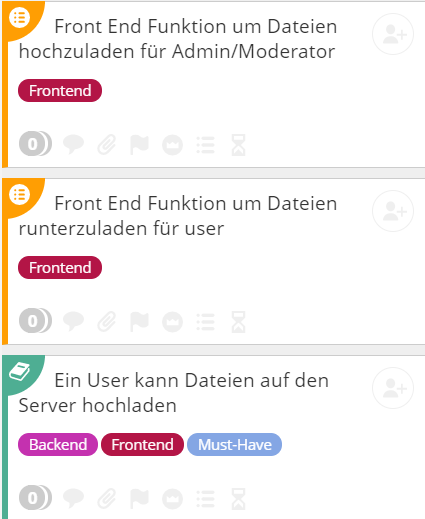
\includegraphics[width=6cm]{User-Story_Tasks.png}
	\caption{Beispiel einer User-Story mit Tasks}
\end{figure}
\end{center}
Nach der Definition wurden allen User-Stories vom Team gemeinsam eine geschätzte Abarbeitungsdauer und eine Priorität zugewiesen.  
User-Stories und die dazugehörigen Tasks wurden dann Sprints hinzugefügt, die eine Dauer von drei Wochen hatten. 
\begin{center}
\begin{figure}[H]
	\centering
	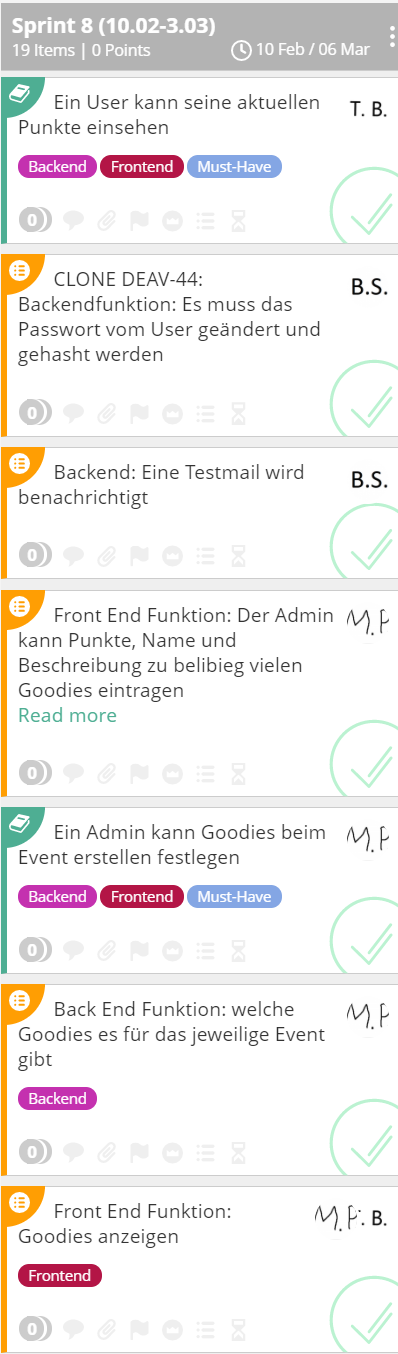
\includegraphics[width=6cm]{Sprint.png}
	\caption{Beispiel eines Sprints}
\end{figure}
\end{center}
Die Diplomarbeitsmitglieder konnten sich zum größten Teil ihre zu bearbeitenden User-Stories selbst aussuchen. Im Falle eines beendeten Sprints, der noch offene User-Stories aufwies, wurden die betroffenen User-Stories wieder zurück in das Product Backlog verschoben und bei Beginn des nächsten Sprints diesem wieder hinzugefügt.
\begin{center}
\begin{figure}[H]
	\centering
	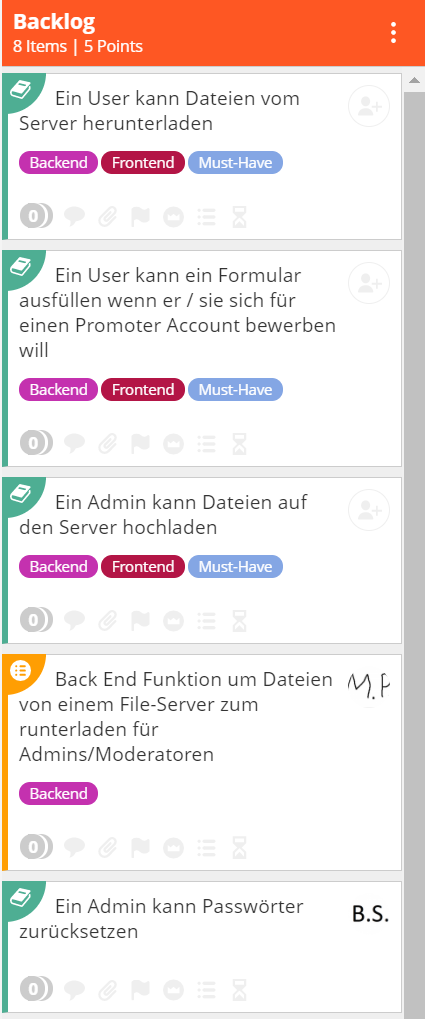
\includegraphics[width=6cm]{product_backlog.png}
	\caption{Product Backlog}
\end{figure}
\end{center}